\beginsong{Roter Wein im Becher}[wuw={Helmut König, Musik nach einem französischen Volkslied}, bo={268}, pfii={15}, pfiii={9}]

\beginverse
\endverse
\centering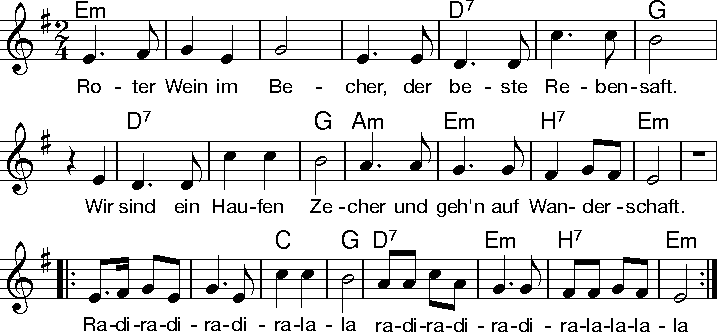
\includegraphics[width=1\textwidth]{Noten/Lied079.pdf}	

\beginverse
\[Em]Morgens bricht die Runde zu \[D7]neuen Fahrten \[G]auf.
Es \[D7]klingt in aller \[G]Mun\[Am]de ein \[Em]frohes \[H7]Liedchen \[Em]auf. 
\endverse

\beginchorus
\lrep Radi, radi, ra-\[C]di rala\[G]la, \[D7]radi, radi, \[Em]ra-di \[H7]ralala\[Em]la. \rrep
\endchorus

\beginverse
^Steine, Staub und Dornen sind ^schwerlich Tippe^lei.
Wir ^müssen uns an^spor^nen, die ^Qual ist ^bald vor^bei.
\endverse

\renewcommand{\everychorus}{\textnote{\bf Refrain (wdh.)}}
\beginchorus
\endchorus
\beginverse
^Treffen wir uns wieder, der ^Zufall nennt den ^Ort,
so ^schallen uns're ^Lie^der in ^weite ^Ferne ^fort.
\endverse
\beginchorus
\endchorus

\endsong

\beginscripture{}
Tippelei = Walz, Gesellenwanderung
\endscripture

\begin{intersong}
\ifthenelse{\boolean{pics}}{
    \vspace{60pt}
    \centering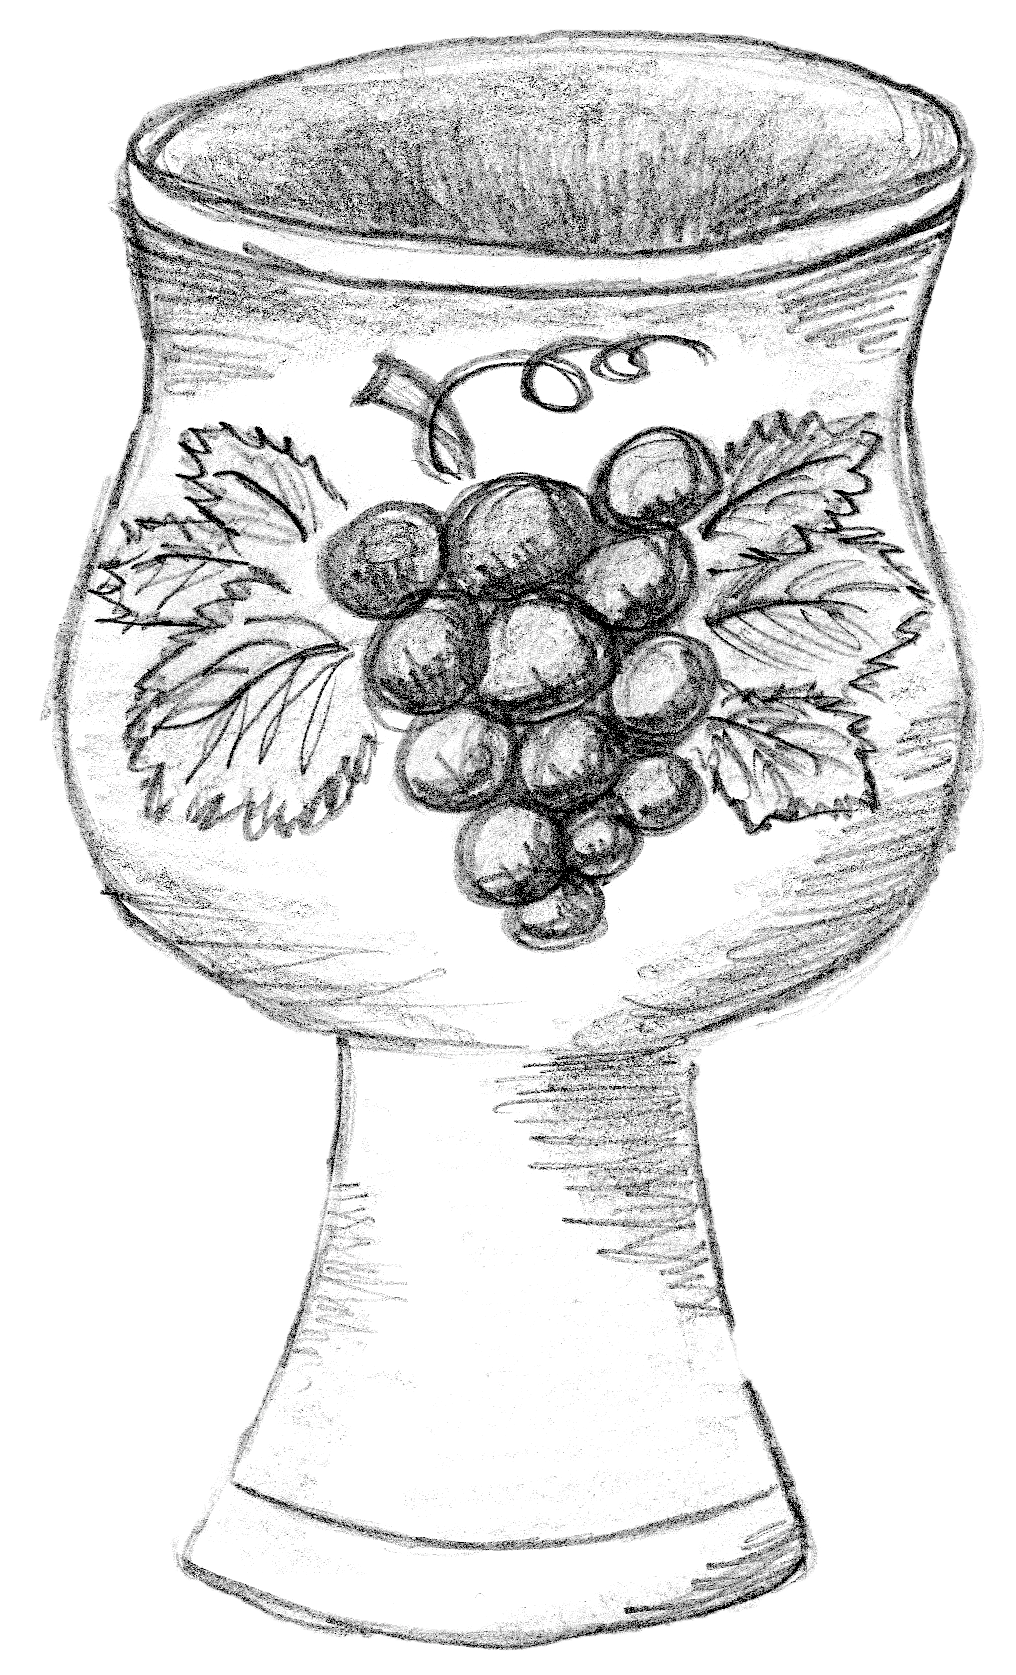
\includegraphics[width=0.6\textwidth]{Bilder/roterwein_irena.png}	
}{}
\end{intersong}